\documentclass[twocolumn,a4paper,10pt]{article}
%\documentclass[a4paper,10pt]{article}
%%%%%%%%%%%%%%%%%%%%%%%%%%%%%%%%%%%%%%%%%%%%%%%%%%%%%%%%%%%%%%%%%%%%%%%%%%%%%%%%%%%%%%%%%%%%

\usepackage{amsmath,amsfonts,amssymb,amsthm}
\usepackage{epsfig}
\usepackage{times}
\usepackage{float}
\usepackage{epsfig}
\usepackage{tikz}
\usepackage{pgfplots}
\usepackage{newpxtext} 
\usepgfplotslibrary{fillbetween}
%\usepackage{subcaption}
\usepackage[small,hang]{caption2}
\usepackage{graphicx}
%\usepackage{showframe}
%
%%%%%%%%%%%%%%%%%%%%
% General layout
%%%%%%%%%%%%%%%%%%%%
%
\setlength{\topmargin}{-5mm}
%\setlength{\topmargin}{0mm}
%\setlength{\evensidemargin}{0mm}
%\setlength{\oddsidemargin}{0mm}
\setlength{\headsep}{0mm}
\setlength{\textheight}{247.0mm}
\setlength{\textwidth}{160mm}
\setlength{\columnsep}{8mm}
\voffset0.0mm\hoffset0.0mm
\parindent5mm
\pagestyle{empty}
%



\makeatletter  



%%%%%%%%%%%%%%%%%%%%
% Sectionning
%%%%%%%%%%%%%%%%%%%%
%
\newcounter{numbersec}
\renewcommand{\section}[1]{\par\noindent\stepcounter{numbersec}
\par
\vspace{6pt}
\noindent\textbf{\large   \arabic{numbersec} \hspace*{0.3cm} #1 }
\par
\vspace{2pt}
}
\renewcommand{\subsection}[1]{
\par
\vspace{6pt}
\noindent\textbf{#1}
\par
}
\renewcommand{\subsubsection}[1]{%
\par
\vspace{6pt}
\textbf{#1.}
}

\newcommand{\norm}[1]{\left\lVert#1\right\rVert}
%
%%%%%%%%%%%%%%%%%%%%
% New commands
%%%%%%%%%%%%%%%%%%%%
%
\newcommand{\Abstract}{\par\vspace{6pt}\noindent\textbf{\large Abstract}\par\vspace{2pt}}
\newcommand{\Acknowledgments}{\par\vspace{6pt}\noindent\textbf{\large Acknowledgments }\par\vspace{2pt}}


\newenvironment{References}{
\par\vspace{6pt}\noindent\textbf{\large References}\par\vspace{2pt}
\begin{small}\begin{list}{ }{
%\itemsep0mm \parsep0mm\settowidth{\labelwidth}{\small\rm 10}\labelsep0mm
\itemsep0mm \parsep0mm\labelsep0mm\leftmargin0mm
%\setlength{\leftmargin}{\labelwidth}}}
}}
{\end{list}\end{small}}


\makeatother

%%%---------------------------------------------------------------------%%%
%%% ------------------- START HERE TO EDIT THE TEXT ------------------- %%%
%%%---------------------------------------------------------------------%%%

%
%%%%%%%%%%%% Insert here the title of the contribution.
%
\title{\vspace*{-12mm}
\LARGE \sc \textbf{  
Study of irregular roughness in minimal channels
}}
%
%%%%%%%%%%%% Insert here the name(s) and address(es) of the author(s).
%
\author{
\Large \bf \textit{ 
J. Yang$^{1}$,
A. Stroh$^{1}$,
S. Jakirli\'c$^{2}$,
B. Frohnapfel$^{1}$ and
P. Forooghi$^{3,}$\footnote{Corresponding author's Email: forooghi@mpe.au.dk}
}  \\ \\
%\bf  \textit{Institute of Fluid Mechanics, Karlsruhe Institute of Technology, Karlsruhe, Germany} \\
\bf  $^{1}$\textit{Institute of Fluid Mechanics, Karlsruhe Institute of Technology, Karlsruhe, Germany} \\
\bf  $^{2}$\textit{Institute of Fluid Mechanics \& Aerodynamics, Technical University Darmstadt,}\\
\bf  \textit{Darmstadt, Germany} \\
\bf  $^{3}$\textit{Dept. Mechanical \& Production Engineering, Aarhus University, Aarhus, Denmark} \\ 

%\\ \underline{\bf alexander.stroh@kit.edu}
}
\date{}



%
%%%%%%%%%%%%%%%%%%%%%%%%%%%%%%%%%%%%%%%%%%%%%%%%%%%%%%%%%%%%%%%%%%%%%%%%%%%%%%%%%%%%%%%%%%%%
\begin{document}
%%%%%%%%%%%%%%%%%%%%%%%%%%%%%%%%%%%%%%%%%%%%%%%%%%%%%%%%%%%%%%%%%%%%%%%%%%%%%%%%%%%%%%%%%%%%
%
%\multicolumn{2}{c}{ffffffffffffffffffffffffffffffffffffffff}

%\begin{multicols}{2}[\section{Titre numgtggggggggggggggggggggggggggggggggggggggggéroté.}]
%   blabla sur deux colonnes, c'est plus sérieux. C'est le
%   style qui est généralement utilisé pour écrire des
%   articles.
%\end{multicols}


%
%\begin{multicols}{1}
%   ffffffffffffffffffffffffffffffffffffffffffffffffffffffffffffffffffffffffffffffffffffffffff
%\end{multicols}

\maketitle
\thispagestyle{empty}

%\multicolumn{2}{\centering}{textddddddddddddddddde}


%\Title{Reconstruction of turbulent fluctuations for hybrid RANS/LES simulations using a synthetic eddy method}
%********** Insert here the name(s) and address(es) of the author(s).
%\Author{A.~Author, A.~N.~Otherauthor}
%\Author{N. Jarrin, R. Prosser, F. Billard and D. Laurence}
%\Address{School of Mechanical, Aerospace and Civil Engineering, }
%\Address{The University of Manchester, Manchester M60 1QD, UK}
%%\Address{$^+$ EDF R\&D, 6 quai Watier, 78420 Chatou, France}
%\Email{ N.Jarrin@postgrad.manchester.ac.uk,  }
%%\Email{ r.prosser@manchester.ac.uk, dominique.laurence@manchester.ac.uk}






%
%%%%%%%%%%%% Insert here the abstract body.
%
\Abstract
Direct numerical simulation (DNS) is carried out to study turbulent flow over irregular rough surfaces in the periodic minimal channel.
A passive scalar is presented in the flow to study heat transfer over rough surfaces with the Prandtl number $Pr=0.7$.
The generation of irregular roughness is based on a mathematical random algorithm, in which the power spectrum (PS) of the roughness height function along with its probability density function (PDF) can be directly prescribed.
The hydro- and thermodynamic properties of the roughness, particularly the roughness function ($\Delta U^+$) as well as the temperature profile offset ($\Delta \Theta^+$), are compared with those obtained from full span DNS for 6 types of roughness topographies with systematically varied PDF and PS configuration at $Re_\tau\approx500$.
The comparison confirms the capability of the minimal channel approach for characterization of irregular rough surfaces providing excellent agreement (within $5\%$) in $\Delta U^+$ and $\Delta \Theta^+$ across various types of roughness topographies.
Results also indicates that random realizations of roughness, with a fixed PS and PDF, translate to similar prediction with a narrow scatter.
Finally, the impact of systematically varied roughness PDF and PS to both velocity and temperature profile is shown.
It is also demonstrated that the influence of varying PDF and PS for roughness skin friction and heat transfer are different.

\section{Introduction}
Rough surfaces are abundant in nature (e.g.  river beds and complex terrain) and engineering (e.g. degraded turbine blades, fouled ship hulls and iced aircraft surfaces). 
It is well established that the topography of roughness can significantly affect its hydrodynamic properties.
In practice, the most important hydrodynamic effect of roughness is an increase in the skin friction coefficient of the surface.
This increase manifests itself in a downward shift in the logarithmic region of inner scaled mean velocity profile $\Delta U^+$.
The shifted velocity profile in logarithmic layer writes:
\begin{equation}
    U^+=\frac{1}{\kappa}\log(y^+)+A_m-\Delta U^+~.
    \label{Ushift}
\end{equation}
Where $\kappa_m\approx0.4$ is the von Karman constant, $A_m$ is the smooth-wall offset.
It is widely reported that $\Delta U^+$ is related to the equivalent sand-grain roughness $k_s$ (Jim\'{e}nez 2004). 
the latter parameter is widely used as an input to engineering applications.
Furthermore, $\Delta U^+=\sqrt{2/C_{fs}}-\sqrt{2/C_{fr}}$ gives direct relation between roughenss function and skin friction (Schultz \& Flack 2009), where $C_{fs}$, $C_{fr}$ are the skin friction coefficients for smooth and rough wall at matched $Re_\tau$ respectively.
Therefore, the central importance of this mean velocity downward shift $\Delta U^+$ in determining the hydrodynamic property of the roughness is understood, which is referred to as the (Hama) roughness function.
To find $\Delta U^+$ for an arbitrary roughness at a certain roughness flow regime, one needs to either run a laboratory (or high-fidelity numerical) experiment or use a so-called roughness correlation, which relates the topography of roughness to $\Delta U^+$. 
While the latter option is obviously less costly, large number of topographical metrics should be systematically investigated to construct such a predictive correlation e.g. skewness $Sk=(1/k_{\text{rms}}^3)\int_S(k-k_{\text{md}})^3\mathrm{d}S$ and $k_{\text{rms}}=\sqrt{(1/S)\int_S(k-k_{\text{md}})^2\mathrm{d}S}$ (Flack \& Schultz 2010), effective slope ES$=(1/S)\int_S|\partial k/\partial x|\mathrm{d}S$ (Napoli \textit{et al.} 2008), roughness correlation length $L_{\text{corr}}$ (Sigal \& Danberg 2008).

Similar to the skin friction, roughness can enhance the heat transfer of the surface, designed roughness are often used in engineering applications (Forooghi \textit{et al.} 2017a).
However, it is widely understood that the enhancement of heat transfer is not directly proportional to the increase of skin friction due to the lack of pressure-drag analog (Dipprey \& sabersky 1963).
This is reflected by the term 'Reynolds analogy factor' $RA=2St/C_f$ (Bons 2005).
Temperature profile of a forced convection smooth-wall flow is demonstrated also exhibits a logarithmic region (Kader 1981). 
The enhancement of heat transfer would result in a downward shift of this logarithmic temperature profile.
Analogous to the Eqn.~\ref{Ushift} The rough wall temperature profile writes:
\begin{equation}
    \frac{\Theta-\Theta_w}{\Theta_\tau}=\frac{1}{\kappa_h}\log(y^+)+A_h(Pr)-\Delta\Theta^+~,
\end{equation}
where $\Theta$ represents the double-averaged temperature field, the offset $A_h$ depends on the molecular Pandtl number $Pr\equiv\nu/\alpha$, $\alpha$ is the thermal diffusivity, $\Theta_w$ is the temperature at wall, $\Theta_\tau$ is the friction temperature $\Theta\equiv(q_w/\rho c_p)/U_\tau$. $q_w$ is the temporally and spatially averaged wall heat flux and $c_p$ is the specific heat at constant pressure.
Thus, the augmentation of heat transfer of a rough wall can be characterized by an analogous term to the roughness function $\Delta U^+$, i.e. $\Delta \Theta^+$.
The heat transfer coefficient of a rough surface, $C_{hr}$, can be derived by $\Delta\Theta^+$ with know $C_{fr}$ at matched $Re_\tau$ through (MacDonald \textit{et al.} 2019):
\begin{equation}
\begin{aligned}
    \Delta \Theta^+=\sqrt{\frac{C_{fs}}{2}}&\bigl(\frac{1}{C_{hs}}-\frac{1}{\kappa_m\kappa_h}\bigr)\\
    &-\sqrt{\frac{C_{fr}}{2}}\bigl(\frac{1}{C_{hr}}-\frac{1}{\kappa_m\kappa_h}\bigr)~.
\end{aligned}
\label{ThetaCh}
\end{equation}
%Unlike the extensive study on the correlation of roughness function $\Delta U^+$, the correlation of $\Delta \Theta^+$ and roughness topography has not received the same amount of attention.

It is since long desired for \textit{a priori} prediction of the aforementioned quantities to get rid of resource demanding (numerical) experiments. 
Flack proposed use of Direct Numerical Simulation (DNS) for generating massive database needed for a universal roughness correlation (Flack 2018).
The major problems in reaching this goal are a) the computational cost of DNS and b) the measurements of realistic rough surfaces are rare and not suitable for systematic studies.
The aim of this work is to examine a new framework, which overcomes both obstacles. To relieve the computational cost we simulate the flow in fully developed turbulent channels with reduced streamwise and spanwise sizes. The idea was previously established and validated by Chung \textit{et al.} (2015), MacDonald \textit{et al.} (2016, 2019) with sinusoidal roughness structure. The criteria of the minimal channel size is given by the authors: $L_z^+\geq\text{max}(100,\Tilde{k}^+/0.4,\lambda_{\text{sin}}^+)$, $L_x^+\geq\text{max}(1000,3L_z^+,\lambda_{\text{sin}}^+)$.
Where $L_x$ and $L_z$ are the streamwise and spanwise extend of the channel, respectively, $\Tilde{k}$ is the amplitude of the sinusoidal structure. $\lambda_{\text{sin}}$ represents the wavelength of the sinusoidal structure.
The criteria are set with the aim of accommodating the minimal channel to the near wall turbulence as well as the roughness structure.
The research shows that minimal channel following the criteria above is capable for this type of roughness (repetitive) structure to predict the roughness function $\Delta U^+$ as well as the temperature offset $\Delta \Theta^+$, but has not been examined for irregular roughness up to now, i.e. the effect of repeating irregular roughness and the limited sample size of roughness topography introduced by the significantly reduced spanwise extend of minimal channel is yet unknown. 

In order to evaluate the validity of this approach for irregular rough surfaces we employ the random algorithm proposed by Pérez-Ràfols \& Almqvist (2019). 
With the roughness generation method surface is generated randomly while the roughness statistical properties can be controlled by its height probability density function (PDF) and the power spectrum (PS) (hence the term pseudo-random roughness).
The generation process is realized by discrete fast Fourier transform (DFFT), thus it is inherently suitable for the DNS simulations where periodic boundary condition is required.

In the present work, pseudo-random roughness with different prescription of PDF and PS are generated and simulated in both minimal channels and conventional full-span channels at $Re_\tau\approx500$.
The performance of the roughness generation method as well as the minimal channels are demonstrated.
The impact of different roughness height PDF and PS configurations on both velocity and temperature fields is exhibited.
%The paper is organized in following way, in~\ref{sec:method} the roughness generation methodology along with the simulation setups will be illustrated. 
%In~\ref{sec:result} simulation results from both minimal channels and full span channels are analyzed.
%Finally in~\ref{sec:Cons} conclusions are given.

\section{Methodology}\label{sec:method}
\subsection{Pseudo-random roughness generation method}
The pseudo-random roughness is generated with the method originally proposed by Pérez-Ràfols \& Almqvist (2019), which will be referred to as generation method for the following text. The roughness structure function $k$ is represented by discrete elevation map on 2-D Cartesian grid, i.e. $k(x,z)$, where $x$, $z$ are the streamwise and spanwise coordinate respectively.
Initially, a roughness map with prescribed roughness PDF is given and is labeled as $k_{\text{PDF}}^0$.
This map do not necessarily contain desired PS.
For the next step, this map is transformed using DFFT and compared with the second initial map with desired PS, which is labeled as $k_{\text{PS}}^0$.
After that, the field is transformed back with inverse DFFT and adjust the height distribution to fit the PDF.
The iterative adjustment of PDF and PS continues until the error, which are measured by the percentage disagreement of PDF and PS profile respectively, approaches a stationary low value.
For further information readers are referred to the literature (Pérez-Ràfols \& Almqvist 2019).
\subsection{Direct numerical simulation}
Direct numerical simulations are carried out in fully developed turbulent channels.
Flow is driven by constant pressure gradient $P_x$.
Periodic boundary condition is applied to the streamwise and spanwise boundaries of the channel.
Upper and lower wall are roughened by the roughness structures.
The roughness with no-slip \& zero-temperature boundary condition is realized by imposing immersed boundary method (IBM) following Goldstein's method (Goldstein 1993).
Where negative external force is applied to the flow in the roughness elements to obtain zero velocity \& temperature inside the roughness. 
An source term $Q=\textbf{u}$ is added to the temperature field to obtain a steady temperature field as the flow flowing through periodic channel and being cooled by the zero-temperature roughness boundaries.
Thus, the Navier-Stokes equation writes:
\begin{equation}
    \nabla\cdot \textbf{u}=0~,
\end{equation}
\begin{equation}
    \frac{\partial \textbf{u}}{\partial t}+\nabla\cdot(\textbf{uu})=-\frac{1}{\rho}\nabla p+\nu\nabla^2\textbf{u}-\frac{1}{\rho}P_x\hat{\mathbf{e_x}}+\textbf{F}_u~,
\end{equation}
\begin{equation}
    \frac{\partial \theta}{\partial t}+\nabla\cdot(\textbf{u}\theta)=\alpha\nabla^2\theta+Q+\textbf{F}_\theta~,
\end{equation}
where \textbf{u} is the velocity vector $\textbf{u}=(u,v,w)^\intercal$, $P_x$ is the mean pressure gradient in the flow direction added as a constant and uniform source term to the momentum equation to drive the flow in the channel. 
Here $p$, $\hat{\mathbf{e_x}}$, $\rho$, $\nu$, $\textbf{F}_\theta$ and $\textbf{F}_u$ are pressure fluctuation, Kronecker delta, density, kinematic viscosity and external source term for momentum and energy equation due to IBM, respectively.
The Friction Reynolds number is defined as $Re_\tau=u_\tau(H-k_{\text{md}})/\nu$, where $u_\tau=\sqrt{\tau_{w}}$ is the friction velocity and $\tau_w=-P_x(H-k_{\text{md}})$ is the wall shear stress controlled by the constant pressure gradient.
\subsection{Description of cases}
Thanks to the flexibility of the roughness generation method, two of the roughness parameters chosen from both PDF and PS sides are systematically varied and analyzed utilizing DNS, namely $Sk $ and the PS slope $p$.
Three values of $Sk$ are selected i.e. $Sk\approx-0.48$, $0$, $0.48$.
Skewed roughness distribution obeys Weibull's distribution $f(k)= K\beta^K k^{(K-1)}e^{-(\beta k)^K}$, where $K$ is the form factor which is adjusted to match desired $Sk$, non-skewed roughness obeys the Gaussian distribution $f(k)=e^{-\frac{1}{2}(\frac{k-\mu}{\sigma})^2}/(1/\sigma\sqrt{2\pi})$.
Moreover the kurtosis $Ku\approx3$ is selected for all roughness in search of the similarity to the Gaussian distribution.
Therefore, the PDF are characterized in terms of negatively skewed, Gaussian and positively skewed distribution.
The height of the roughness is scaled by the the 99\% confidence interval of the PDF, which is denoted as $k_{99}$.
$k_{99}=0.1H$ is prescribed to all roughness configurations.
In order to avoid extreme high/low roughness, roughness elements locate out side $1.2\times k_{99}/2$ around the meltdown height $k_{md}=(1/S)\int_Sk\mathrm{d}S$ are excluded, where $S$ is the wall-normal projection area of the surface.

On the other side, power-law PS is employed, i.e. $E_k(\textbf{q})=C_0(\norm{\textbf{q}}/q_0)^p$, where \textbf{q} is the wavenumber vector $\textbf{q}=(q_x,q_z)^\intercal$, $q_0=2\pi/\lambda_0$ is the referencing wavenumber corresponding to the largest in-plane length scale $\lambda_0$, $C_0$ is a constant to scale the roughness height, and $p$ is the slope of the power-law PS.
$p$ is chosen as $-1$ and $-2$ in seek of overlapping with previous researches (Barros \textit{et al.} 2018, Nikora \textit{et al.} (2019)).
The cutoff wavelengths of the PS are selected to be moderate to the channel size as well as the grid resolution, i.e. the presenting roughness wavelength $\lambda$ obeys $0.8H\leq\lambda\leq0.08H$.

In summary, by "grid searching" of these two roughness parameters in two channel sizes, in total 12 ($3\times2\times2$) rough surfaces are individually produced.
Following abbreviation is used throughout the text to distinguish the cases:
\begin{equation}
    \overbrace{\underbrace{\boxed{\;G\;}}_\text{PDF}\;\;\underbrace{\boxed{ \;2\;}}_\text{$-p$} }^{\text{Topography}}\;|\overbrace{\boxed{\;F\;}}^{\text{Channel size}}~.
\end{equation}
\begin{itemize}
\setlength\itemsep{0em}
    \item The first character indicates the type of PDF; $G$ for Gaussian distribution, $P$ for positively skewed ($Sk\approx0.48$), and $N$ for negatively skewed ($Sk\approx-0.48$).
    \item The second digit indicates the PS slope; $1$ for $p=-1$ and $2$ for $p=-2$.
    \item The following character(s) indicates the channel size; $F$ for full channel ($8H\times4H$), $M$ for the minimal channel ($2.4H\times0.8H$)
\end{itemize}
One of the irregular roughness topographies, $G2F$, is illustrated in figure~\ref{G24F}, the size of the minimal channel is represented by the black frame in the figure.
The roughness metrics that are widely used for roughness characterization are shown in Table~\ref{tab:SumOfCase}.
As one can see, the roughness topographical statistics from the random generation process are preserved for both surface sizes.
It is worth mentioning that the roughness for minimal channels and full span channels are independently generated, which means each surface has an individual realization but the statistics are controlled by the generation method.
Thus, the stability of the generation method is demonstrated in terms of roughness topographical statistics.

%\begin{figure}
%    \centering
%    \begin{subfigure}{0.5\textwidth}
%    \input{tikz/HPDG14F.tikz}
%    \end{subfigure}
%    \begin{subfigure}{.5\textwidth}
%        \centering
%        \input{tikz/PSforp}
%    \end{subfigure}
%    \caption{Caption}
%    \label{fig:my_label}
%\end{figure}
    \begin{table*}[hh]
        \centering
        \begin{tabular}{cccccccc|cc}
            Topography & $Sk$ & $p$ &$k_{\text{md}}/H$&$k_{\text{rms}}/H$&$L_x^{\text{corr}}/H$&$S_f/S$&ES&$\Delta U^+$&$\Delta \Theta^+$\\[3pt]
            $P1F$ & $0.48$ & $-1$ &0.046&0.0208&0.052&0.28&0.57&7.33&4.70\\
            $P1M$ & $0.48$ & $-1$ &0.046&0.0208&0.056&0.28&0.55&7.28&4.72\\[3pt]
            $P2F$ & $0.48$ & $-2 $&0.046&0.0208&0.100&0.21&0.44&6.99&3.93\\
            $P2M$ & $0.48$ & $-2 $&0.046&0.0208&0.110&0.20&0.40&6.86&4.37\\[3pt]
            $G1F$ & $0$    & $-1$ &0.061&0.0200&0.050&0.27&0.54&6.67&3.93\\
            $G1M$ & $0$    & $-1$ &0.061&0.0200&0.054&0.27&0.53&6.66&3.99\\[3pt]
            $G2F$ & $0$    & $-2$ &0.061&0.0200&0.100&0.20&0.43&6.30&3.62\\
            $G2M$ & $0$    & $-2$ &0.061&0.0200&0.108&0.19&0.40&6.39&3.70\\[3pt]
            $N1F$ & $-0.48$ & $-1$&0.074&0.0208&0.052&0.28&0.57&6.14&4.73\\
            $N1M$ & $-0.48$ & $-1$&0.074&0.0208&0.056&0.28&0.55&6.07&4.68\\[3pt]
            $N2F$ & $-0.48$ & $-2$&0.074&0.0208&0.100&0.21&0.44&5.82&4.44\\
            $N2M$ & $-0.48$ & $-2$&0.074&0.0208&0.110&0.20&0.40&5.63&4.38\\
        \end{tabular}
                \caption{Roughness topographical statistics, where  $S_f$ is the total frontal projected area of the roughness. $L_x^{\text{corr}}$ refers to the length scale where the roughness auto-correlation in streamwise direction drops under 0.2. Simulation results are shown on the last two columns on the left.}
        \label{tab:SumOfCase}
    \end{table*}
%The grid size for DNS is mostly determined by the smallest in-plane roughness wavelength, $\lambda_1=0.08H$.
%In order to properly model each roughness elements with IBM, based on the mesh independent test approximately 8 computational cells are used for each roughness element, which lead to the simulation resolution $N_x\times N_y\times N_z=900\times401\times480$ and $256\times401\times96$ for full span channel and minimal channel, respectively.
\begin{figure}[h]
\centering
%{\includegraphics[width=0.8\textwidth,trim=0 0cm 2.5cm 0, clip]{png/roughness.png}}
\begin{tikzpicture}
\pgfplotsset{
    scale only axis,
 colormap={RWB}{
rgb255=(0,0,255)
rgb255=(255,255,225)
rgb255=(255,0,0)
        }
}
\begin{axis}[
		xlabel={$L_x/H$},
		ylabel={$L_z/H$},
		unit vector ratio=1 1 1,
		xmin=0,xmax=8,
		ymin=0,ymax=4,
		y dir=reverse,
		clip=true,
		set layers,
		clip mode=individual,
		width=.65\linewidth,
				ylabel near ticks,
		xtick={0,2,...,8},
		ytick={0,2,...,4},
		label style={font=\footnotesize},
		tick label style={font=\footnotesize},
		colorbar,
		point meta min=0,
		point meta max=0.1226,
		colorbar style={
			xlabel={$k/H$},
			xlabel shift = 10.5 pt,
		ytick={0,0.12},
		width=0.2cm
		}
	]
	\centering
\addplot [thick, color=blue, on layer=axis background]
graphics[xmin=0,ymin=0,xmax=8,ymax=4]{png/G24Fc.png};
	\draw[color=black,thick] (0, 0) rectangle (axis cs: 2.4, 0.8);
\end{axis}
\end{tikzpicture}
\caption{Full-span roughness sample $G2F$. The black rectangle represents the size of the minimal channel. Color bar shows the surface height.}
\label{G24F}
\end{figure} 



\section{Results}\label{sec:result}
The DNS results, especially the mean velocity and temperature profiles, $\bigl<\overline{u}\bigr>(y)$ and $\bigl<\overline{\theta}\bigr>(y)$ are obtained by applying double-averaging method: $\bigl<\overline{\Phi}\bigr>(y)=\frac{1}{S}\iint_S\overline{\Phi}(x,y,z)\mathrm{d}x\mathrm{d}z$.
Where $\overline{\Phi}(x,y,z)$ is the time averaged velocity $\Bar{u}$ /temperature $\Bar{\theta}$ field. The angular brackest $\bigl<\cdot\bigr>$ denotes horizontal averaging.
The double-averaged velocity and temperature profiles will be denoted as $U$ and $\Theta$, respectively.

Furthermore, due to the fluctuating surface structure the origin of the wall normal coordinate of a rough surface cannot be naturally defined.
In order to align the logarithmic layer of smooth and rough surfaces, zero plane displacement $d$ is considered.
To this end, Jackson (1981) proposed use of moment centroid of the drag profile on rough surfaces as the virtual origin for the logarithmic velocity profile.
The definition of the zero plane displacement $d$ in present work follows Jackson's method.
%It is also shown in the present work that $d$, derived from velocity field, also applies for temperature field.
\subsection{Effect of channel size}
\begin{figure}[h]
	\centering
	        \begin{tikzpicture}[]
        \centering
        \begin{axis}[
            ylabel={$U^+$},
            xlabel={$(y-d)^+$},
            ymin=0, ymax=35,
			xmin=1,xmax=500,
            width=1\linewidth,
            height=0.7\linewidth,
			xmode=log,
					ylabel near ticks,
			ytick={0,10,20,30},
            legend style={fill=white,font=\tiny,anchor=north east},
            legend pos=north east,
            label style={font=\footnotesize},
            tick label style={font=\footnotesize}
            ]
            						\addplot [
            black,thick,dashed,mark=none,
            ]
            coordinates{
            (160, 40)
            (160, -15)
            };
            \addlegendentry{critical height $y_c$}
			\addplot [
            green,solid,thick,
            ]
            table [x=X, y=Y,col sep=comma]{CSV/UprofileG24FM7.csv};
            \addlegendentry{$G2M$}
						\addplot [
            red,solid,thick,
            ]
            table [x=X, y=Y,col sep=comma]{CSV/UprofileG24FM8.csv};
            \addlegendentry{$G2F$}
						\addplot [
            black,dashdotted,thick,
            ]
            table [x=X, y=Y,col sep=comma]{CSV/UprofileG24FM9.csv};
            \addplot [
            red,dashed,thick,
            ]
            table [x=X, y=Y,col sep=comma]{CSV/UprofileG24FM3.csv};
            \addplot [
            green,dashed,thick,
            ]
            table [x=X, y=Y,col sep=comma]{CSV/UprofileG24FM4.csv};	            
        \end{axis}
        
        \begin{axis}[
		%xlabel=$(y-d)^+$,
		ylabel={$U^+_s-U^+_r$},
		xmin=0,xmax=500,
		ymin=0,ymax=8,
		%y dir=reverse,
		clip=true,
		set layers,
		xmode=log,
		clip mode=individual,
	    height=0.45\linewidth,
		width=.45\linewidth,
		ylabel near ticks,
		xlabel near ticks,
		%axis x line*=bottom,
		%axis y line*=left,
		%xticklabels=\empty,
		%ytick={0.12},
		label style={font=\footnotesize},
		yticklabel style={/pgf/number format/fixed},
		tick label style={font=\footnotesize},
		at={(0.13\linewidth,0.22\linewidth)}
	]
	\centering
\addplot [
            black,thick,dashed,
            ]
            coordinates{
            (160,-4)
            (160,10)
            };
									\addplot [
            green,solid,thick,
            ]
            table [x=X, y=Y,col sep=comma]{CSV/DUprofileG24mf24.csv};
						\addplot [
            red,solid,thick,
            ]
            table [x=X, y=Y,col sep=comma]{CSV/DUprofileG24mf25.csv};


\end{axis}
        
        \end{tikzpicture}
	\caption{Mean velocity profile of roughness type $G2$, dashed line: velocity profile of smooth wall $U^+_s$, solid line: velocity profile of rough wall $U^+_r$. The inset shows the velocity retardation $U^+_s-U^+_r$ as a function of wall normal distance $(y-d)^+$.}
	\label{UG241}
\end{figure}
%\begin{figure}[H]
%    \centering
%	        \begin{tikzpicture}[]
        \centering
        \begin{axis}[
            ylabel={$\Delta U^+$},
            xlabel={$(y-d)^+$},
            ymin=-2, ymax=8,
			xmin=1,xmax=500,
            width=1.\linewidth,
            height=0.8\linewidth,
			xmode=log,
            legend style={fill=white,font=\tiny,anchor=south east},
            legend pos= south east,
            label style={font=\footnotesize},
            tick label style={font=\footnotesize}
            ]
\addplot [
            black,thick,dashed,
            ]
            coordinates{
            (160,-4)
            (160,10)
            };
            \addlegendentry{critical height $y_c$}
									\addplot [
            green,solid,thick,
            ]
            table [x=X, y=Y,col sep=comma]{CSV/DUprofileG24mf24.csv};
            \addlegendentry{$G2M$}
						\addplot [
            red,solid,thick,
            ]
            table [x=X, y=Y,col sep=comma]{CSV/DUprofileG24mf25.csv};
            \addlegendentry{$G2F$}


        \end{axis}
        \end{tikzpicture}
%	\caption{Velocity offset profile of roughness type $G2$}
%\label{UG242}
%\end{figure}
The velocity field of exemplary cases $G$2$M$ and $G$2$F$ are compared in figure~\ref{UG241}.
The velocity offset profiles $U_s^+-U_r^+$ are shown in the inset of figure~\ref{UG241} using same coloring style.
With the same measurement, temperature fields predicted by minimal channel and full span channel are compared in figure~\ref{TG241}.
As one can observe, excellent agreement of the profiles are achieved between minimal channels and full span channels below each critical height $y_c$.
Due to the nature of minimal channels, sudden increase of the profiles in outer layer can be observed for both smooth and rough cases.
However, the offset profiles of minimal channel and full span channel, as shown in the inset, collapse well and reach constant values in logarithmic layer.
The roughness function $\Delta U^+$ as well as $\Delta \Theta^+$ are obtained by measuring the mean offset of the profile in logarithmic layer, specifically over $y^+=160-250$.
\begin{figure}[h]
	\centering
	        \begin{tikzpicture}[]
        \centering
        \begin{axis}[
            ylabel={$\Theta^+$},
            xlabel={$(y-d)^+$},
            ymin=0, ymax=35,
			xmin=1,xmax=500,
            width=1\linewidth,
            height=0.8\linewidth,
			xmode=log,
					ylabel near ticks,
			ytick={0,10,20,30},
            legend style={fill=white,font=\tiny,anchor=north east},
            legend pos=north east,
            label style={font=\footnotesize},
            tick label style={font=\footnotesize}
            ]
                    						\addplot [
            black,thick,dashed,
            ]
            coordinates{
            (160,0)
            (160,200)
            };
                        \addlegendentry{critical height $y_c$}
                        						\addplot [
            green,solid,thick,
            ]
            table [x=X, y=Y,col sep=comma]{CSV/TprofileG243.csv};
            \addlegendentry{$G2M$}
						\addplot [
            red,solid,thick,
            ]
            table [x=X, y=Y,col sep=comma]{CSV/TprofileG244.csv};
            \addlegendentry{$G2F$}
            \addplot [
            red,dashed,thick,
            ]
            table [x=X, y=Y,col sep=comma]{CSV/TprofileG241.csv};
			\addplot [
            green,dashed,thick,
            ]
            table [x=X, y=Y,col sep=comma]{CSV/TprofileG242.csv};



        \end{axis}
        
        
                \begin{axis}[
		%xlabel=$(y-d)^+$,
		ylabel={$\Theta^+_s-\Theta^+_r$},
		xmin=0,xmax=500,
		ymin=0,ymax=8,
		%y dir=reverse,
		clip=true,
		set layers,
		xmode=log,
		clip mode=individual,
	    height=0.45\linewidth,
		width=.45\linewidth,
		ylabel near ticks,
		xlabel near ticks,
		%axis x line*=bottom,
		%axis y line*=left,
		%xticklabels=\empty,
		%ytick={0.12},
		label style={font=\footnotesize},
		yticklabel style={/pgf/number format/fixed},
		tick label style={font=\footnotesize},
		at={(0.13\linewidth,0.32\linewidth)}
	]
	\centering
                                						\addplot [
            black,thick,dashed,
            ]
            coordinates{
            (160,-5)
            (160,8)
            };
            \addplot [
            green,solid,thick,
            ]
            table [x=X, y=Y,col sep=comma]{CSV/DTprofile1.csv};
									\addplot [
            red,solid,thick,
            ]
            table [x=X, y=Y,col sep=comma]{CSV/DTprofile2.csv};
\end{axis}
        \end{tikzpicture}
	\caption{Mean temperature profile of roughness type $G2$, dashed line: temperature profile of smooth wall $\Theta^+_s$, solid line: temperature profile of rough wall $\Theta^+_r$. The inset shows the temperature retardation $\Theta^+_s-\Theta^+_r$ as a function of wall normal distance $(y-d)^+$.}
	\label{TG241}
\end{figure}
    \begin{figure}[h]
        \centering
                \begin{tikzpicture}[]
        \centering
        \begin{axis}[
            ylabel={$\frac{\Delta U_{\text{M}}^+}{\Delta U_{\text{F}}^+}$, $\frac{\Delta \Theta_{\text{M}}^+}{\Delta \Theta_{\text{F}}^+}$},
            xlabel={$\Delta U_{\text{F}}^+$, $\Delta \Theta_{\text{F}}^+$},
            ymin=0.8,
            ymax=1.2,
			xmax=8.4,
			xmin=3,
					ylabel near ticks,
			%xtick={-2,-1.5,...,-0.4},
            width=1\linewidth,
            height=.7\linewidth,
            label style={font=\footnotesize},
            legend style={font=\tiny,anchor=south west},
                        legend pos=south west,
            tick label style={font=\footnotesize}
            ]
			\addplot [
            black,only marks,mark=o,
            ]
            coordinates{
            (6.67,6.66/6.67)
            (6.30,6.39/6.30)
            (7.33,7.28/7.33)
            (6.99,6.86/6.99)
            (6.14,6.07/6.14)
            (5.82,5.63/5.82)
            };
			\addlegendentry{$\Delta U^+$}
			\addplot [
            black,only marks,mark=square,
            ]
            coordinates{
            (4.17,4.19/4.17)
            (3.82,3.84/3.82)
            (3.93,3.99/3.97)
            (3.62,3.72/3.62)
            (3.87,3.80/3.87)
            (3.54,3.49/3.54)
            };
			\addlegendentry{$\Delta \Theta^+$}
			

%						\addplot [
%            gray,only marks,mark=square,
%            ]
%            coordinates{
%            (6.30, 6.46/6.30)
%            (6.30, 6.42/6.30)
%            (6.30, 6.56/6.30)
%            (6.30, 6.58/6.30)
%            (6.30, 6.58/6.30)
%            (6.30, 6.19/6.30)
%            (6.30, 6.54/6.30)
%            (6.30, 6.30/6.30)
%            };
%			\addlegendentry{$G24M2-500s$}
						\addplot [
            red,thick,solid,mark=square,
            ]
            coordinates{
            (0, 1)
            (9, 1)
            };
						\addplot [
            gray,thick,dashed,mark=square,
            ]
            coordinates{
            (0, 1.05)
            (9, 1.05)
            };
            						\addplot [
            gray,thick,dashed,mark=square,
            ]
            coordinates{
            (0, 0.95)
            (9, 0.95)
            };
			\node[red,right] at (axis cs: 7.6,1.03) {\tiny $\pm5\%$};

        \end{axis}
        \end{tikzpicture}
        \caption{$\Delta U^+_{M}$ and $\Delta \Theta^+_{M}$ predicted by minimal channels normalized by full span channel prediction $\Delta U^+_{F}$ and $\Delta \Theta^+_{F}$, respectively $\circ$: $\Delta U^+$, $\square$: $\Delta \Theta^+$. Gray dashed lines indicate the boundary of 5\% error interval around $\Delta U_{M}^+/\Delta U_{F}^+=\Delta \Theta_{M}^+/\Delta \Theta_{F}^+$=1}
        \label{DUDT}
    \end{figure}
    
Generalizing the observation to all considered cases, $\Delta U^+$ along with $\Delta \Theta^+$ are summarized on the last two columns in table.~\ref{tab:SumOfCase}.
To visualize the disagreement of minimal channel with full span channel, graphical comparison are illustrated in figure~\ref{DUDT}.
It can be observed that minimal channels show excellent agreement with the conventional full span channels, the discrepancies of both $\Delta U^+$ and $\Delta \Theta^+$ lie under 5\%.
Consistent predictions indicate the capability of the minimal channels in reproducing the hydro- and thermodynamic properties of the irregular pseudo-realistic roughness.
%Notably, rough surfaces for full span and minimal channels are independently generated through random roughness generation process, thus the realizations of the roughness are unique, only the statistic properties, i.e. roughness PS and PDF, are controlled by the generation process. 
The results imply the determining characters of the roughness PS and PDF to both skin friction and heat transfer. 
%\begin{table}
%\centering
%    \begin{tabular}{c| c c |  c c}
%    & $\Delta U^+$& &$\Delta \Theta^+$\\[3pt]
%     Case&$F$&$M$&$F$&$M$\\[3pt]
%    $P1$&7.33&7.28&4.70&4.72\\
%    $P2$&6.99&6.86&4.37&4.39\\[3pt]
%     $G1$&6.67&6.66&3.93&3.99\\
%     $G2$&6.30&6.39&3.62&3.70\\ [3pt]
%    $N1$&6.14&6.07&4.73&4.68\\
%    $N2$&5.82&5.63&4.44&4.38\\
%    \end{tabular}
%    \caption{Summary of roughness function $\Delta U^+$ (left) and temperature offset %$\Delta \Theta^+$ (right) at $Re_\tau\approx500$.}
%    \label{ResultAll}
%    \end{table}


\subsection{Effect of roughness topography}
\begin{figure}[h]
    \centering
            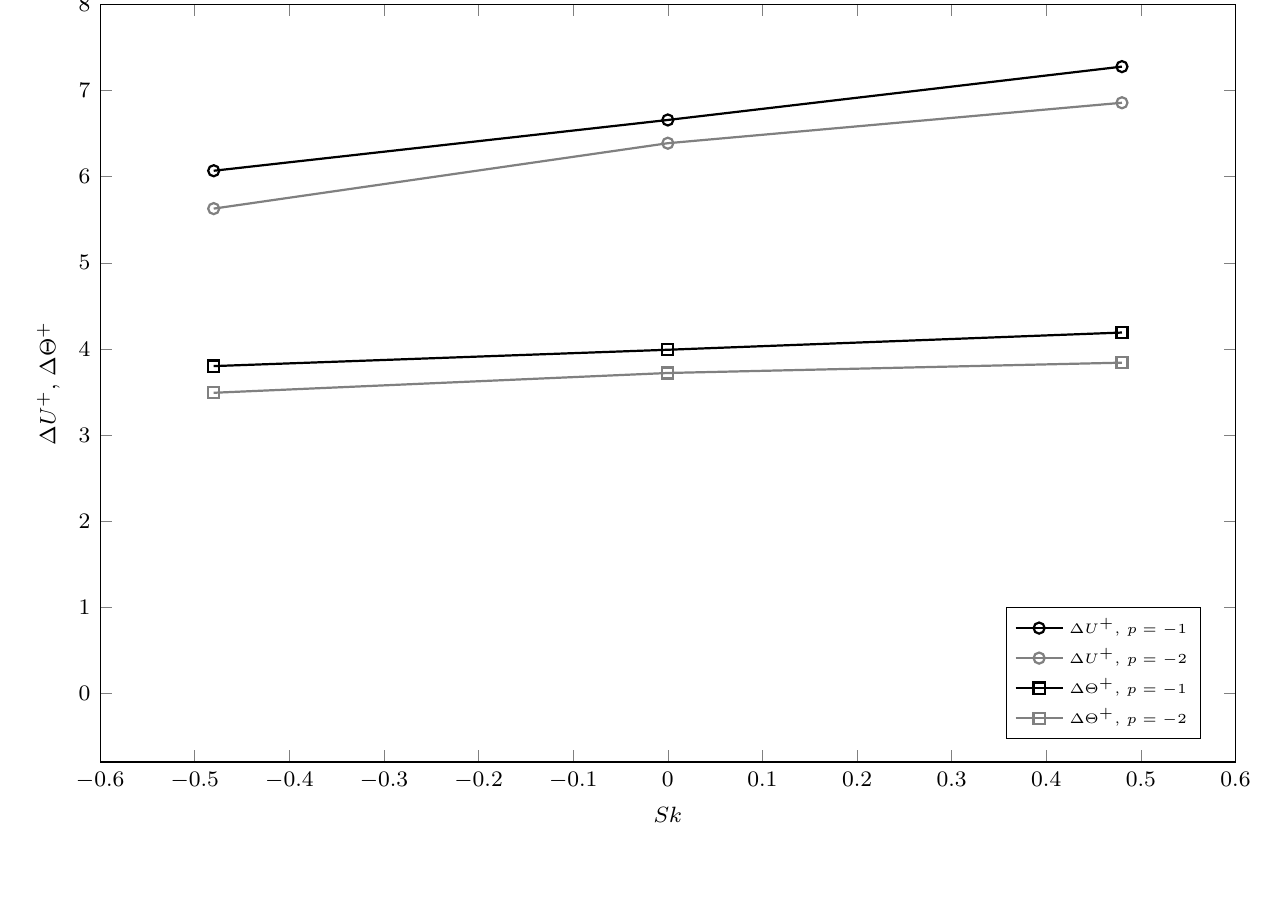
\begin{tikzpicture}
        \centering
        \begin{axis}[
            ylabel={$\Delta U^+$, $\Delta \Theta^+$},
            xlabel={$Sk$},
            ymin=-0.8, ymax=8,
			xmax=0.6,
			xmin=-0.60,
					ylabel near ticks,
            width=1\linewidth,
            height=0.7\linewidth,
            label style={font=\footnotesize},
            legend style={font=\tiny,anchor=south east},
                        legend pos=south east,
            tick label style={font=\footnotesize}
            ]
			\addplot [
            black,thick,mark=o,
            ]
            coordinates{
            (0.48, 7.28)
            (0, 6.66)
            (-0.48,6.07)
            };
			\addlegendentry{$\Delta U^+$, $p=-1$}
						\addplot [
            gray,thick,mark=o,
            ]
            coordinates{
            (0.48, 6.86)
            (0, 6.39)
            (-0.48,5.63)
            };
			\addlegendentry{$\Delta U^+$, $p=-2$}
					\addplot [
            black,thick,mark=square,
            ]
            coordinates{
            (0.48, 4.19)
            (0, 3.99)
            (-0.48,3.80)
            };
			\addlegendentry{$\Delta \Theta^+$, $p=-1$}
						\addplot [
            gray,thick,mark=square,
            ]
            coordinates{
            (0.48, 3.84)
            (0, 3.72)
            (-0.48,3.49)
            };
			\addlegendentry{$\Delta \Theta^+$, $p=-2$}
        \end{axis}
        \end{tikzpicture}
    \caption{$\Delta U^+$(circles) and $\Delta \Theta^+$(squares) predictions from minimal channels. Black: $p=-1$, gray: $p=-2$.}
    \label{fig:DUTOPO}
\end{figure}
\begin{figure}[h]
    \centering
            \begin{tikzpicture}
        \centering
        \begin{axis}[
            ylabel={$\Delta U^+$, $\Delta \Theta^+$},
            xlabel={ES},
            ymin=3, ymax=8,
			xmax=0.74,
			xmin=0.4,
					ylabel near ticks,
            width=1\linewidth,
            height=0.7\linewidth,
            label style={font=\footnotesize},
            legend style={font=\tiny,anchor=south east},
                        legend pos=south east,
            tick label style={font=\footnotesize}
            ]
                        			\addplot [
            blue,thick,mark=none
            ]
            coordinates{
            (0.57, 4.19)
            (0.44, 3.84)
            };
            			\addlegendentry{$Sk=0.48$}
            			\addplot [
            red,thick,mark=none
            ]
            coordinates{
            (0.54,3.99)
            (.43,3.70)
            };
            \addlegendentry{$Sk=0$}
            			\addplot [
            green,thick,mark=none
            ]
            coordinates{
            (.57,3.80)
            (.44,3.49)
            };
            \addlegendentry{$Sk=-0.48$}
            			\addplot [
            blue,thick,mark=o
            ]
            coordinates{
            (0.57, 7.28)
            (0.44, 6.86)
            };
            			\addplot [
            red,thick,mark=o
            ]
            coordinates{
            (0.54,6.66)
            (.43,6.39)
            };
            			\addplot [
            green,thick,mark=o
            ]
            coordinates{
            (.57,6.07)
            (.44,5.63)
            };
            
            
            
			\addplot [
            blue,thick,mark=square
            ]
            coordinates{
            (0.57, 4.19)
            (0.44, 3.84)
            };
            			\addplot [
            red,thick,mark=square
            ]
            coordinates{
            (0.54,3.99)
            (.43,3.70)
            };
            			\addplot [
            green,thick,mark=square
            ]
            coordinates{
            (.57,3.80)
            (.44,3.49)
            };

        \end{axis}
        \end{tikzpicture}
    \caption{$\Delta U^+$(circles) and $\Delta \Theta^+$(squares) predictions from minimal channels. Blue: $Sk=0.48$, red: $Sk=0$, green: $Sk=-0.48$.}
    \label{fig:DTTOPO}
\end{figure}
Given the satisfactory performance of minimal channel simulations, in the following content the prediction results by minimal channels will be analysed.
An overview of the roughness function $\Delta U^+$ from minimal channel simulations is plotted in figure~\ref{fig:DUTOPO}, where roughness function $\Delta U^+$ is shown as a function of skewness $Sk$, grouped by the PS slope $p$.
As investigated by Flack \textit{et al.}(2020), positively skewed rough surfaces give higher skin friction than non-skewed or negatively skewed roughness.
Negatively skewed surfaces show 'slip-velocity' effect (Jelly \& Busse 2018), which translates into a weaker mean velocity retardation.
The trend observed in the present results fully agrees with what suggested by the previous researchers.

On the other hand, the averaged offset of logarithmic temperature profile $\Delta \Theta^+$, analogous to $\Delta U^+$, are shown in figure~\ref{fig:DTTOPO}.
The evolution of $\Delta \Theta^+$ show significant difference to $\Delta U^+$ -- both in value and trend.
It is demonstrated that Gaussian surfaces show lowest interference to temperature field while these skewed roughness, regardless of its sign, can enhance the temperature offset.
By adjusting the PS slope $p$ the shift of $\Delta \Theta^+$ can be observed for all roughness topographies.
To shed light into the correlation of spatial roughness distribution and $\Delta \Theta^+$, $\Delta \Theta^+$ is plotted as a function of effective slope ES in figure~\ref{fig:DTTOPO}.
Approximately parallel increases of $\Delta \Theta^+$ with ES for all types of roughness are exhibited.
Similar trend can be found for $\Delta U^+$.
Notably, surfaces whose $Sk=\pm0.48$ show comparable value of $\Delta\Theta^+$.
The exemplary temperature profiles of $P2M$, $G2M$ and $N2M$ are ploted in figure~\ref{GPN}.
In the near wall region, due to the different blockage effect introduced by skewness, temperature profiles diverge.
However in the logarithmic layer, the temperature profiles of positively and negatively skewed roughness collapse.
Have to mention that identical $\Delta \Theta^+$ of negatively and positibely skewed roughness do not necessarily translate to a identical $C_{hr}$ according to Eqn.~\ref{ThetaCh}.
Detailed study of the effect of skewness on the heat transfer coefficient should be carried out.
\begin{figure}
        \begin{tikzpicture}[]
        \centering
        \begin{axis}[
            ylabel={$\Theta^+$},
            xlabel={$(y-d)^+$},
            ymin=0, ymax=15,
			xmin=1,xmax=500,
            width=1\linewidth,
            height=0.7\linewidth,
			xmode=log,
					ylabel near ticks,
			ytick={0,5,10,15},
            legend style={fill=white,font=\tiny,anchor=north west},
            legend pos=north west,
            label style={font=\footnotesize},
            tick label style={font=\footnotesize}
            ]       
                                    \addplot [
            blue,solid,thick,
            ]
            table [x=X, y=Y,col sep=comma]{CSV/GPNM1_T3.csv};	            \addlegendentry{$Sk=0.48$}
             
                        \addplot [
            red,solid,thick,
            ]
            table [x=X, y=Y,col sep=comma]{CSV/GPNM1_T1.csv};	
            \addlegendentry{$Sk=0$}
                                    \addplot [
            green,solid,thick,
            ]
            table [x=X, y=Y,col sep=comma]{CSV/GPNM1_T2.csv};	
      \addlegendentry{$Sk=-0.48$}
                          						\addplot [
            black,thick,dashed,
            ]
            coordinates{
            (160,0)
            (160,200)
            };
                  \addlegendentry{critical height $y_c$}
        \end{axis}
       
        \end{tikzpicture}
\caption{Temperature profiles of $G/P/N2M$}
\label{GPN}
\end{figure}
\section{ Conclusions }\label{sec:Cons}
DNS is carried out for fully developed turbulent flow over artificial irregular roughness driven by constant pressure gradient at $Re_\tau\approx 500$.
A source term for temperature field is applied while the temperature for the roughness is prescribed to be 0.
The rough surfaces are generated based on the mathematical roughness generation method proposed by Ràfols \& Almqvist(2019).
With the generation method roughness with desired PDF and PS can be generated.
3 types of PDF, namely $Sk=-0.48$, $0$, $0.48$ are combined with 2 types of power-law PS inputs whose slope $p=-1$\& $-2$.
First of all, the performance of the roughness generation method is assessed by showing the statistics of independently generated surfaces for full span channel and minimal channel.
It is demonstrated that the minimal channel is capable for reproducing the hydro- and thermodynamic properties of the artificial irregular roughness with significant reduction of computational effort.
In the present work, roughness function $\Delta U^+$ and the offset of temperature profile in logarithmic layer $\Delta T^+$ are compared among all types of roughness topographies with systematically adjusted PDF and PS.
It is found that the influence of roughness is different for skin friction and heat transfer.
A monotonically increase of $\Delta U^+$ as a function of $Sk$ is observed, while for temperature field the skewed roughness -- regard less peak or pit dominant -- can enhance the heat transfer to an comparable extent relative to non-skewed roughness with identical PS.
General increase of $\Delta U^+$ and $\Delta\theta^+$ is reported when the PS slope $p$ is steeper.
Parallel increase of skin friction and heat transfer for different types of roughness can be observed with increasing ES.

%%%%%%%%%% Insert here acknowledgments if necessary

\Acknowledgments

Jiasheng Yang and Pourya Forooghi gratefully acknowledge financial support from Friedrich und Elisabeth Boysen-Foundation (BOY-151). This work was performed on the supercomputer ForHLR and the storage facility LSDF funded by the Ministry of Science, Research and the Arts Baden-Württemberg and by the Federal Ministry of Education and Research.


%%%%%%%%%%%%%%%%%%%%%%%%%%%%%%%%%%%%%%%%%%%%%%%%%%%%%%%%%%%%%%%%%%%%%%%
%%%%%%%%%%%%%%%%%%%%%%%%%%%%%%%%%%%%%%%%%%%%%%%%%%%%%%%%%%%%%%%%%%%%%%%
%
\begin{References}
\item Jim\'{e}nez, J. (2004), Turbulent flows over rough walls, {\it Ann. Rev. Fluid Mech.} Vol. 36, pp. 173-196.
\item Flack, K. A. (2018), Moving beyond Moody, {\it  J. Fluid Mech.}, Vol. 842, pp. 1-4.
\item Chung, D., Chan, L., MacDonald, L., Hutchins, N. and Ooi, A. (2015), A fast direct numerical simulation method for characterising hydraulic roughness, {\it  J. Fluid Mech.}, Vol. 773, pp. 418-431.
\item Pérez-Ràfols, F. and Almqvist, A. (2019), Generating randomly rough surfaces with given height probability distribution and power spectrum, {\it Tribology International}, Vol. 131, pp. 591-604.
\item Flack, K. A. and Schultz, M. P. (2010), Review of Hydraulic Roughness Scales in the Fully Rough Regime, {\it J. Fluids Engineering}, Vol. 132.
\item Napoli, E., Armenio, V. and De Marchis, M (2008). The effect of the slope of irregularly distributed roughness elements on turbulent wall-bounded flows, {\it  J. Fluid Mech.}, Vol. 613. pp. 385-394.
\item MacDonald, M., Chung, D. Hutchins, N., Chan, L., Ooi, A. and Garc{\'{\i}}a-Mayoral, A. (2016), The minimal channel: a fast and direct method for characterising roughness, {\it Journal of Physics: Conference Series}, Vol. 708,
\item Sigal, A., Danberg, J. E. (2008), New correlation of roughness density effect on the turbulent boudnary layer, {\it AIAA Journal}, Vol. 28, pp. 554-556.
\item Goldstein, D., Handler, R. and Sirovich, L., Modeling a no-slip flow boundary with an external force field., {\it Journal of Computational Physics}, Vol. 105, pp. 354-366.
\item Forooghi, P., Flory, M., Bertsche, D., Wetzel, T. and Frohnapfel, B. (2017a). Heat transfer enhancement on the liquid side of an industrially designed flat-tube heat exchanger with passive insertes-numerical investigation. {\it Appl. Therm. Eng.}, Vol. 123, pp. 573-583.
\item Bons, J.P. (2005) A critical assessment of Reynolds analogy for turbine flows. {\it ASME J. Heat Transf.}, Vol. 127(5), pp. 472-485.
\item Kader, B. A. (1981) Temperature and concentration profiles in fully turbulent boundary layers. {\it Intl. J. Heat Mass Transfer}, Vol. 24, pp. 1541-1544.
\item Cebeci, T. and Bradshaw, P. (1984), Physical and computational aspects of convective heat transfer. Springer. 
\item MacDonald, M., Hutchins, N., Chung, D. (2019), Roughness effects in turbulent forced convection, {\it J. Fluid Mech.}, Vol. 861, pp. 138-162.
\item Barros, J. M., Schultz, M. P. and Flack, K. A. (2018), Measurements of skin-friction of systematically generated surfaces roughness,{\it  Intl. J. Heat and Fluid Flow}, Vol. 72, pp. 1-7.
\item Nikora, V. I., Stoesser, T., Cameron, S. M., Stewart, M., Papadopoulos, K., Ouro, P., McSherry, R.,Zampiron, A., Marusic, I., Falconer, R. A. and et al (2019), Friction factor decomposition for rough-wall flows: theoretical background and application to open-channel flows, {\it J. Fluid Mech.}, Vol. 872, pp. 626-664.
\item Flack, K.A., Schultz. M.P. \& Barros, J.M. 2020 Skin friction measurements systematically-varied roughness: Probing the role of roughness amplitude and skewness. \textit{Flow, Turbulence and Combustion}, Vol. 104, pp.317-329.
\item Jelly, T.O. \& Busse, A. 2018 Reynolds and dispersive shear stress contributions above highly skewed roughness \textit{J. Fluid Mech.} vol. 852, pp. 710-724.
\item Jackson, P.S. 1981 On the displacement height in the logarithmic velocity profile. \textit{J. Fluid Mech.} vol.111, pp.15-25.
\end{References}
%
%
\end{document}